\section{Detailkonzept} \label{sec:detailkonzept}

Das Konzept mit den Wasserliften ist am besten geeignet für unsere Anwendung. Es existieren bereits solche «Rohrkettenförderer», die jedoch Produkte hinaufbefördern. Wir nutzen dieses System um das Wasser nach unten zu befördern und dabei Energie zu gewinnen. Es werden insgesamt sechs Lifte benötigt. Fünf Lifte überwinden je 60.08\si{m} und der unterste Lift überwindet 80.24\si{m}. In der Abbildung \ref{fig:PrinzipGrobkonzept4} \nameref{fig:PrinzipGrobkonzept4} ist dies grafisch dargestellt.

\subsection{Elektronik}

\begin{figure}[H]
\centering
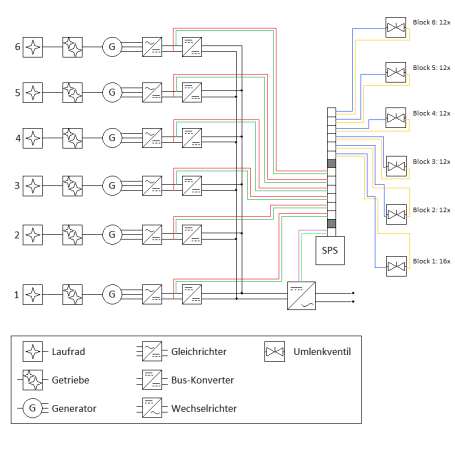
\includegraphics[width=\linewidth]{Skizze_GK4.png}
\caption{Prinzipschema}
\label{fig:Prinzipschema}
\end{figure}

\paragraph{Funktionsbeschreibung}
Die potentielle Energie des Abwassers wird über ein Laufrad in kinetische Energie umgewandelt. Mittels eines Getriebes wird die vom Laufrad kommende Drehzahl dem Generator angepasst, dieser wandelt die kinetische Energie in elektrische um. Der Gleichrichter transformiert den 3 Phasen Drehstrom in einen 2 poligen Gleichstrom. Um Rückkoppelungen auf dem DC-Bus zu vermeiden schalten wir zwischen den Gleichrichter und den DC-Bus einen Bus-Konverter. Die summierte Energie aller sechs Generatorenstränge wird über einen Wechselrichter ins Stromnetz eingespeist.
Zur Überwachung und auch zur Ansteuerung der Umlenkventile im Wartungsfall wird eine SPS verwendet.


%TODO Michel: Bild (Michel) mit allen Komponenten abgebildet einfügen. Kurze Beschreibung mit Verweis auf bild

\paragraph{Generator}

%TODO Lars: Tagesgangkurve beschreiben und dadurch mindestleitung Generator (3kW) begründen: (Tagesenergie 191.1MJ)

\begin{figure}[H]
\centering
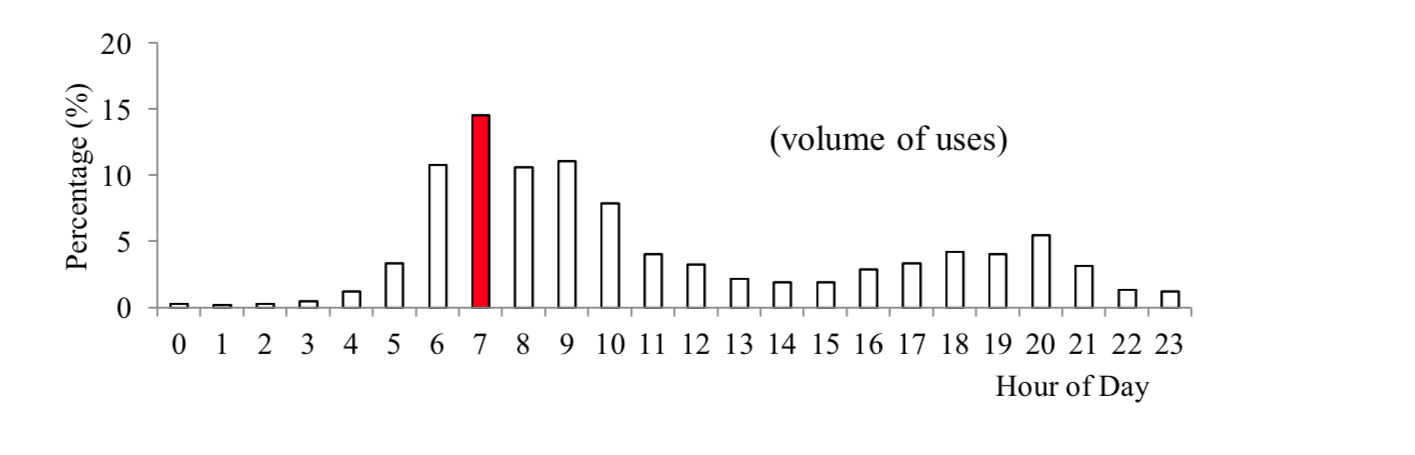
\includegraphics[width=\linewidth]{tagesGangKurve.png}
\caption{Typische Tagesgangkurve. \cite{peakWaterDemand}}
\label{fig:tagesGangKurve}
\end{figure}

%TODO Lars: Ausgesuchter Generator mit Kosten auflisten; Warum dieser Generator?

\paragraph{Wechselrichter}

%TODO Lars: Ausgesuchter Wechselrichter mit Kosten auflisten; Warum dieser Wechselrichter?

\paragraph{DC-DC Wandler}

%TODO Lars: Ausgesuchter DC-DC Wandler mit Kosten auflisten; Warum dieser DC-DC Wandler(Kein Strom darf zurückfliessen!)?

\paragraph{Wechselrichter}

%TODO Roni: Kosten einfügen; Kann die Leistung die Angezeigt wird auch auf einen PC übertragen werden? Kommunikationsschnittstelle? Unterster Abschnitt nochmals überarbeiten


Damit die gewonnen Leistung in das Netz eingespiesen werden kann, muss der Wechselrichter folgende Eigenschaften aufweisen. 

\textbf{Leistung:}		9KW \newline
\textbf{Ausgang:}		3Phasen \newline
\textbf{Kosten:}		Die Kosten sollen möglichst gering gehalten werden. \newline

In der Förderungsanlage wird ein Asynchrongenerator verbaut. Die Firma Voltacon ist bekannt für ihre Hochleistungswechselrichter.

Das Model Hybrid Wechselrichter HSI10000 entspricht den gewünschten Anforderungen für unsere Förderungsanlage. Der Wechselrichter transformiert die 48VDC auf 230VAC mit einer Frequenz von 50\si{\hertz}. Das Gerät kann bis zu einer Leistung von 10KW erbringen. Mittels integrierten Displays kann die erbrachte Leistung zusätzlich abgelesen werden. 

Gemäss Datenblatt lassen die Ströme regeln bis 200A. 
Der Wechselrichter hat einen Netzunabhängigen Energiespeicher der mittels Batterie geladen werden könnte (Batterie-Backup). Für die die Kommunikation sind verschieden Optionen vorhanden wie über den USB Port, RS-232 oder den SNMP (Simple Network Management Protocol) Überwachungssoftware für Echtzeitstatusanzeige und-steuerung.

Kosten: 3'401\si{Fr}


\paragraph{Kontrollsystem}

%TODO Lars: Kontrollsystem in Worte Fassen: 

%SPS Beckhof besitzt: 
%1 Kontrollerklemme BK9050 (200.-)
%20 Digitale Ausgangsklemmen KL1114 (1 Klemme = 100.-)	;Für Ventile schalten
%20 Digitale Eingangsklemmen KL2134 (1 Klemme = 100.-)	;Für überprüfen ob Ventile geschaltet ist
%7 AnalogEingangsklemmen KL3162 (1 Klemme = 100.-)		;Strommessung über hochohmigen widerstand
%1 Abschlussklemme KL9010 (50.-)

%IndustriePC suchen (Um die 1000.-)


\newpage


\subsection{Mechanik}

\paragraph{Rohrkette}

In der Industrie werden Rohrkettenförderer für den Transport von Schuttgüter verwendet. In der Abbildung \ref{fig:Rohrkettenfoerderer} \nameref{fig:Rohrkettenfoerderer} ist der Innenaufbau eines solchen Rohrkettenförderers ersichtlich.

\begin{figure} [H]
	\centering
	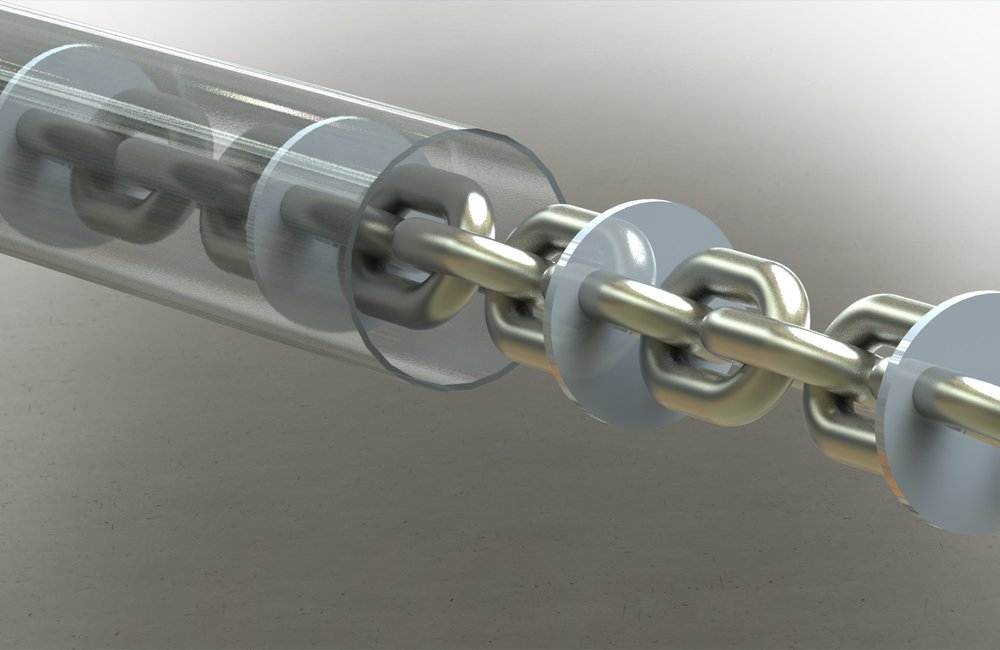
\includegraphics[width=6cm]{Rohrkettenfoerderer.jpg}
	\caption{Innenaufbau Rohrkettenförderer \cite{abconvey}}
	\label{fig:Rohrkettenfoerderer}
\end{figure}

Wir wollen keinen Schutt nach oben befördern, daher muss dieses System auf unsere Anforderungen angepasst werden. Diese Anforderungen sind, dass die verwendeten Materialien Robust gegenüber Korrasion sind, da das Abwasser aggressiv auf diese wirkt. Weiter müssen, um einen möglichst hohen Wirkungsgrad zu erreichen, die Platten mit möglichst kleinem Spielraum zur Ausserwand konstruiert werden, damit das Wasser nicht einfach auf der Seite herunterfliessen kann und gleichzeitig nicht eine zu grosse Reibung erzeugt wird. Die Drehachse, an dem der Generator angeschlossen wird ist ein Stösselkettenrad. Dieser ist in der Abbildung \ref{fig:stoesselkettenrad} \nameref{fig:stoesselkettenrad} zu sehen

\begin{figure} [H]
	\centering
	\includegraphics[width=6cm]{Stoesselkettenrad.jpg}
	\caption{Stösselkettenrad \cite{schrage}}
	\label{fig:stoesselkettenrad}
\end{figure}


Um diesen Wasserlift zu bauen beauftragen wir die Firma Schrage, ein führender Speziallist für Rohrketten, die in Deutschland zu Hause ist, beauftragt. Die Kosten belaufen sich für die 60.08\si{m} Höhendifferenz auf ca. 10'000\si{Fr} pro Lift und für die 80.24\si{m} Höhendifferenz auf ca. 13'000\si{Fr}. Insgesamt würde die Analage mit den Rohrketten, Rohr und Stösselkettenrad ca.63'000\si{Fr} kosten. \cite{schrage}

\newpage

\paragraph{Zahnradsytem}
%TODO Lars: Mindestdrehzahl dem Generator anpassen. Raddurchmesser für den Richtiungswechsel der rohrketten. Einen guten Wert annehmen

\paragraph{Ventile}

%TODO Roni: Ventile aussuchen die das Wasser entweder in die Falleitung oder in das rohrketten rohr leitet


\subsection{Kosten}

%TODO Sonntag: Alle Kosten zusammentragen